\documentclass[twoside]{book}

% Packages required by doxygen
\usepackage{fixltx2e}
\usepackage{calc}
\usepackage{doxygen}
\usepackage[export]{adjustbox} % also loads graphicx
\usepackage{graphicx}
\usepackage[utf8]{inputenc}
\usepackage{makeidx}
\usepackage{multicol}
\usepackage{multirow}
\PassOptionsToPackage{warn}{textcomp}
\usepackage{textcomp}
\usepackage[nointegrals]{wasysym}
\usepackage[table]{xcolor}

% Font selection
\usepackage[T1]{fontenc}
\usepackage[scaled=.90]{helvet}
\usepackage{courier}
\usepackage{amssymb}
\usepackage{sectsty}
\renewcommand{\familydefault}{\sfdefault}
\allsectionsfont{%
  \fontseries{bc}\selectfont%
  \color{darkgray}%
}
\renewcommand{\DoxyLabelFont}{%
  \fontseries{bc}\selectfont%
  \color{darkgray}%
}
\newcommand{\+}{\discretionary{\mbox{\scriptsize$\hookleftarrow$}}{}{}}

% Page & text layout
\usepackage{geometry}
\geometry{%
  a4paper,%
  top=2.5cm,%
  bottom=2.5cm,%
  left=2.5cm,%
  right=2.5cm%
}
\tolerance=750
\hfuzz=15pt
\hbadness=750
\setlength{\emergencystretch}{15pt}
\setlength{\parindent}{0cm}
\setlength{\parskip}{3ex plus 2ex minus 2ex}
\makeatletter
\renewcommand{\paragraph}{%
  \@startsection{paragraph}{4}{0ex}{-1.0ex}{1.0ex}{%
    \normalfont\normalsize\bfseries\SS@parafont%
  }%
}
\renewcommand{\subparagraph}{%
  \@startsection{subparagraph}{5}{0ex}{-1.0ex}{1.0ex}{%
    \normalfont\normalsize\bfseries\SS@subparafont%
  }%
}
\makeatother

% Headers & footers
\usepackage{fancyhdr}
\pagestyle{fancyplain}
\fancyhead[LE]{\fancyplain{}{\bfseries\thepage}}
\fancyhead[CE]{\fancyplain{}{}}
\fancyhead[RE]{\fancyplain{}{\bfseries\leftmark}}
\fancyhead[LO]{\fancyplain{}{\bfseries\rightmark}}
\fancyhead[CO]{\fancyplain{}{}}
\fancyhead[RO]{\fancyplain{}{\bfseries\thepage}}
\fancyfoot[LE]{\fancyplain{}{}}
\fancyfoot[CE]{\fancyplain{}{}}
\fancyfoot[RE]{\fancyplain{}{\bfseries\scriptsize Generated by Doxygen }}
\fancyfoot[LO]{\fancyplain{}{\bfseries\scriptsize Generated by Doxygen }}
\fancyfoot[CO]{\fancyplain{}{}}
\fancyfoot[RO]{\fancyplain{}{}}
\renewcommand{\footrulewidth}{0.4pt}
\renewcommand{\chaptermark}[1]{%
  \markboth{#1}{}%
}
\renewcommand{\sectionmark}[1]{%
  \markright{\thesection\ #1}%
}

% Indices & bibliography
\usepackage{natbib}
\usepackage[titles]{tocloft}
\setcounter{tocdepth}{3}
\setcounter{secnumdepth}{5}
\makeindex

% Hyperlinks (required, but should be loaded last)
\usepackage{ifpdf}
\ifpdf
  \usepackage[pdftex,pagebackref=true]{hyperref}
\else
  \usepackage[ps2pdf,pagebackref=true]{hyperref}
\fi
\hypersetup{%
  colorlinks=true,%
  linkcolor=blue,%
  citecolor=blue,%
  unicode%
}

% Custom commands
\newcommand{\clearemptydoublepage}{%
  \newpage{\pagestyle{empty}\cleardoublepage}%
}

\usepackage{caption}
\captionsetup{labelsep=space,justification=centering,font={bf},singlelinecheck=off,skip=4pt,position=top}

%===== C O N T E N T S =====

\begin{document}

% Titlepage & ToC
\hypersetup{pageanchor=false,
             bookmarksnumbered=true,
             pdfencoding=unicode
            }
\pagenumbering{alph}
\begin{titlepage}
\vspace*{7cm}
\begin{center}%
{\Large L\+I2\+P\+L2\+G8 }\\
\vspace*{1cm}
{\large Generated by Doxygen 1.8.13}\\
\end{center}
\end{titlepage}
\clearemptydoublepage
\pagenumbering{roman}
\tableofcontents
\clearemptydoublepage
\pagenumbering{arabic}
\hypersetup{pageanchor=true}

%--- Begin generated contents ---
\chapter{G\+R\+U\+PO 8 / P\+L2 / M\+I\+EI}
\label{md_README}
\Hypertarget{md_README}
\section*{Relatório Guião 5}

Divisão do projeto em 3 módulos. Camada de dados\+: Definição de um conjunto de funções que retornam elementos do estado e funções de consulta do estado de modo a trabalhar com os dados. Lógica do programa\+: Criação da função jogar fazendo condições com as funções da camada de dados. Interface \+: Interpretação dos dados do tabuleiro, imprimir o tabuleiro e ir jogando com lendo do teclado as jogadas até aparecer uma jogada inválida. Dificuldades\+: Criação de todas as funções da camada de dados na medida em que foram criadas a medida que se construia a lógica do programa e a interface, ou seja, quando existia uma necessidade.

\#\+Membros\+: Davi Carneiro Pereira -\/ a22854 João Tadeu Correia Torres -\/ a85846 Tiago Lucas Alves -\/ a93261 
\chapter{Class Index}
\section{Class List}
Here are the classes, structs, unions and interfaces with brief descriptions\+:\begin{DoxyCompactList}
\item\contentsline{section}{\hyperlink{structCOORDENADA}{C\+O\+O\+R\+D\+E\+N\+A\+DA} \\*Tipo de dados para as coordenadas }{\pageref{structCOORDENADA}}{}
\item\contentsline{section}{\hyperlink{structESTADO}{E\+S\+T\+A\+DO} \\*Tipo de dados para o estado }{\pageref{structESTADO}}{}
\item\contentsline{section}{\hyperlink{structJOGADA}{J\+O\+G\+A\+DA} \\*Tipo de dados para a jogada }{\pageref{structJOGADA}}{}
\item\contentsline{section}{\hyperlink{structnodo}{nodo} }{\pageref{structnodo}}{}
\end{DoxyCompactList}

\chapter{File Index}
\section{File List}
Here is a list of all documented files with brief descriptions\+:\begin{DoxyCompactList}
\item\contentsline{section}{\hyperlink{controller_8h}{controller.\+h} }{\pageref{controller_8h}}{}
\item\contentsline{section}{\hyperlink{data_8h}{data.\+h} }{\pageref{data_8h}}{}
\item\contentsline{section}{\hyperlink{interface_8h}{interface.\+h} }{\pageref{interface_8h}}{}
\end{DoxyCompactList}

\chapter{Class Documentation}
\hypertarget{structCOORDENADA}{}\section{C\+O\+O\+R\+D\+E\+N\+A\+DA Struct Reference}
\label{structCOORDENADA}\index{C\+O\+O\+R\+D\+E\+N\+A\+DA@{C\+O\+O\+R\+D\+E\+N\+A\+DA}}


Tipo de dados para as coordenadas.  




{\ttfamily \#include $<$data.\+h$>$}

\subsection*{Public Attributes}
\begin{DoxyCompactItemize}
\item 
\mbox{\Hypertarget{structCOORDENADA_adfbc8d4856ce807139fdf62e00aed29a}\label{structCOORDENADA_adfbc8d4856ce807139fdf62e00aed29a}} 
int {\bfseries coluna}
\item 
\mbox{\Hypertarget{structCOORDENADA_aefe14bcc5a066ac3b21500cc3d28c06f}\label{structCOORDENADA_aefe14bcc5a066ac3b21500cc3d28c06f}} 
int {\bfseries linha}
\end{DoxyCompactItemize}


\subsection{Detailed Description}
Tipo de dados para as coordenadas. 

The documentation for this struct was generated from the following file\+:\begin{DoxyCompactItemize}
\item 
\hyperlink{data_8h}{data.\+h}\end{DoxyCompactItemize}

\hypertarget{structESTADO}{}\section{E\+S\+T\+A\+DO Struct Reference}
\label{structESTADO}\index{E\+S\+T\+A\+DO@{E\+S\+T\+A\+DO}}


Tipo de dados para o estado.  




{\ttfamily \#include $<$data.\+h$>$}



Collaboration diagram for E\+S\+T\+A\+DO\+:\nopagebreak
\begin{figure}[H]
\begin{center}
\leavevmode
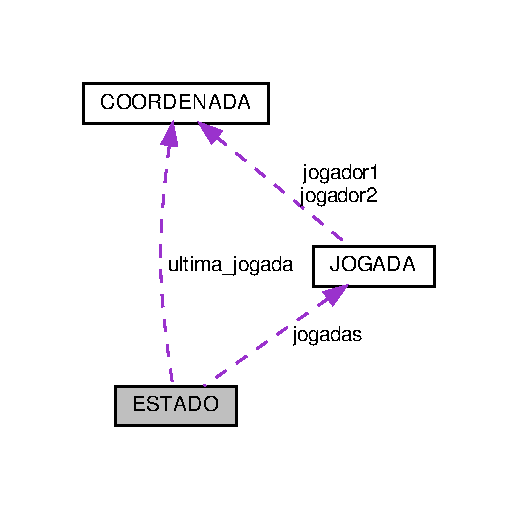
\includegraphics[width=249pt]{structESTADO__coll__graph}
\end{center}
\end{figure}
\subsection*{Public Attributes}
\begin{DoxyCompactItemize}
\item 
\hyperlink{data_8h_aba91601f16d4c485b2d9b8c429f27039}{C\+A\+SA} \hyperlink{structESTADO_ab56f0f1be16954d3768b4174d14c087d}{tab} \mbox{[}8\mbox{]}\mbox{[}8\mbox{]}
\item 
\hyperlink{data_8h_a94c221d29a1760f008b7834093259b7d}{J\+O\+G\+A\+D\+AS} \hyperlink{structESTADO_afae43b87a488fad0f2b56a18bad31d18}{jogadas}
\item 
int \hyperlink{structESTADO_a261495728744647e618b4e623f5a4b7a}{num\+\_\+jogadas}
\item 
int \hyperlink{structESTADO_a1dbc6b513f27065f40d17af021699015}{pointer\+\_\+jogada}
\item 
int \hyperlink{structESTADO_a5dd28e2e68b7aef2b6b7ea88e02eff58}{jogador\+\_\+atual}
\item 
int \hyperlink{structESTADO_adf1064dfc09145b6995a7897249f1674}{num\+\_\+comando}
\item 
\hyperlink{structCOORDENADA}{C\+O\+O\+R\+D\+E\+N\+A\+DA} \hyperlink{structESTADO_a4896a5c5c1f40b43fb795623327e3f47}{ultima\+\_\+jogada}
\end{DoxyCompactItemize}


\subsection{Detailed Description}
Tipo de dados para o estado. 

\subsection{Member Data Documentation}
\mbox{\Hypertarget{structESTADO_afae43b87a488fad0f2b56a18bad31d18}\label{structESTADO_afae43b87a488fad0f2b56a18bad31d18}} 
\index{E\+S\+T\+A\+DO@{E\+S\+T\+A\+DO}!jogadas@{jogadas}}
\index{jogadas@{jogadas}!E\+S\+T\+A\+DO@{E\+S\+T\+A\+DO}}
\subsubsection{\texorpdfstring{jogadas}{jogadas}}
{\footnotesize\ttfamily \hyperlink{data_8h_a94c221d29a1760f008b7834093259b7d}{J\+O\+G\+A\+D\+AS} E\+S\+T\+A\+D\+O\+::jogadas}

As jogadas \mbox{\Hypertarget{structESTADO_a5dd28e2e68b7aef2b6b7ea88e02eff58}\label{structESTADO_a5dd28e2e68b7aef2b6b7ea88e02eff58}} 
\index{E\+S\+T\+A\+DO@{E\+S\+T\+A\+DO}!jogador\+\_\+atual@{jogador\+\_\+atual}}
\index{jogador\+\_\+atual@{jogador\+\_\+atual}!E\+S\+T\+A\+DO@{E\+S\+T\+A\+DO}}
\subsubsection{\texorpdfstring{jogador\+\_\+atual}{jogador\_atual}}
{\footnotesize\ttfamily int E\+S\+T\+A\+D\+O\+::jogador\+\_\+atual}

O jogador atual \mbox{\Hypertarget{structESTADO_adf1064dfc09145b6995a7897249f1674}\label{structESTADO_adf1064dfc09145b6995a7897249f1674}} 
\index{E\+S\+T\+A\+DO@{E\+S\+T\+A\+DO}!num\+\_\+comando@{num\+\_\+comando}}
\index{num\+\_\+comando@{num\+\_\+comando}!E\+S\+T\+A\+DO@{E\+S\+T\+A\+DO}}
\subsubsection{\texorpdfstring{num\+\_\+comando}{num\_comando}}
{\footnotesize\ttfamily int E\+S\+T\+A\+D\+O\+::num\+\_\+comando}

O nº de comando, usado no prompt \mbox{\Hypertarget{structESTADO_a261495728744647e618b4e623f5a4b7a}\label{structESTADO_a261495728744647e618b4e623f5a4b7a}} 
\index{E\+S\+T\+A\+DO@{E\+S\+T\+A\+DO}!num\+\_\+jogadas@{num\+\_\+jogadas}}
\index{num\+\_\+jogadas@{num\+\_\+jogadas}!E\+S\+T\+A\+DO@{E\+S\+T\+A\+DO}}
\subsubsection{\texorpdfstring{num\+\_\+jogadas}{num\_jogadas}}
{\footnotesize\ttfamily int E\+S\+T\+A\+D\+O\+::num\+\_\+jogadas}

O número das jogadas, usado no prompt \mbox{\Hypertarget{structESTADO_a1dbc6b513f27065f40d17af021699015}\label{structESTADO_a1dbc6b513f27065f40d17af021699015}} 
\index{E\+S\+T\+A\+DO@{E\+S\+T\+A\+DO}!pointer\+\_\+jogada@{pointer\+\_\+jogada}}
\index{pointer\+\_\+jogada@{pointer\+\_\+jogada}!E\+S\+T\+A\+DO@{E\+S\+T\+A\+DO}}
\subsubsection{\texorpdfstring{pointer\+\_\+jogada}{pointer\_jogada}}
{\footnotesize\ttfamily int E\+S\+T\+A\+D\+O\+::pointer\+\_\+jogada}

O apontador para a jogada atual \mbox{\Hypertarget{structESTADO_ab56f0f1be16954d3768b4174d14c087d}\label{structESTADO_ab56f0f1be16954d3768b4174d14c087d}} 
\index{E\+S\+T\+A\+DO@{E\+S\+T\+A\+DO}!tab@{tab}}
\index{tab@{tab}!E\+S\+T\+A\+DO@{E\+S\+T\+A\+DO}}
\subsubsection{\texorpdfstring{tab}{tab}}
{\footnotesize\ttfamily \hyperlink{data_8h_aba91601f16d4c485b2d9b8c429f27039}{C\+A\+SA} E\+S\+T\+A\+D\+O\+::tab\mbox{[}8\mbox{]}\mbox{[}8\mbox{]}}

O tabuleiro \mbox{\Hypertarget{structESTADO_a4896a5c5c1f40b43fb795623327e3f47}\label{structESTADO_a4896a5c5c1f40b43fb795623327e3f47}} 
\index{E\+S\+T\+A\+DO@{E\+S\+T\+A\+DO}!ultima\+\_\+jogada@{ultima\+\_\+jogada}}
\index{ultima\+\_\+jogada@{ultima\+\_\+jogada}!E\+S\+T\+A\+DO@{E\+S\+T\+A\+DO}}
\subsubsection{\texorpdfstring{ultima\+\_\+jogada}{ultima\_jogada}}
{\footnotesize\ttfamily \hyperlink{structCOORDENADA}{C\+O\+O\+R\+D\+E\+N\+A\+DA} E\+S\+T\+A\+D\+O\+::ultima\+\_\+jogada}

A coordenada da última jogada 

The documentation for this struct was generated from the following file\+:\begin{DoxyCompactItemize}
\item 
\hyperlink{data_8h}{data.\+h}\end{DoxyCompactItemize}

\hypertarget{structJOGADA}{}\section{J\+O\+G\+A\+DA Struct Reference}
\label{structJOGADA}\index{J\+O\+G\+A\+DA@{J\+O\+G\+A\+DA}}


Tipo de dados para a jogada.  




{\ttfamily \#include $<$data.\+h$>$}



Collaboration diagram for J\+O\+G\+A\+DA\+:
% FIG 0
\subsection*{Public Attributes}
\begin{DoxyCompactItemize}
\item 
\mbox{\Hypertarget{structJOGADA_a93d9306cb0c49b66b7d9a615bffe0149}\label{structJOGADA_a93d9306cb0c49b66b7d9a615bffe0149}} 
\hyperlink{structCOORDENADA}{C\+O\+O\+R\+D\+E\+N\+A\+DA} {\bfseries jogador1}
\item 
\mbox{\Hypertarget{structJOGADA_ab46b16dfbdc7f2af9430c8dcdac0914b}\label{structJOGADA_ab46b16dfbdc7f2af9430c8dcdac0914b}} 
\hyperlink{structCOORDENADA}{C\+O\+O\+R\+D\+E\+N\+A\+DA} {\bfseries jogador2}
\end{DoxyCompactItemize}


\subsection{Detailed Description}
Tipo de dados para a jogada. 

The documentation for this struct was generated from the following file\+:\begin{DoxyCompactItemize}
\item 
\hyperlink{data_8h}{data.\+h}\end{DoxyCompactItemize}

\chapter{File Documentation}
\hypertarget{controller_8h}{}\section{controller.\+h File Reference}
\label{controller_8h}\index{controller.\+h@{controller.\+h}}
{\ttfamily \#include \char`\"{}data.\+h\char`\"{}}\newline
Include dependency graph for controller.\+h\+:\nopagebreak
\begin{figure}[H]
\begin{center}
\leavevmode
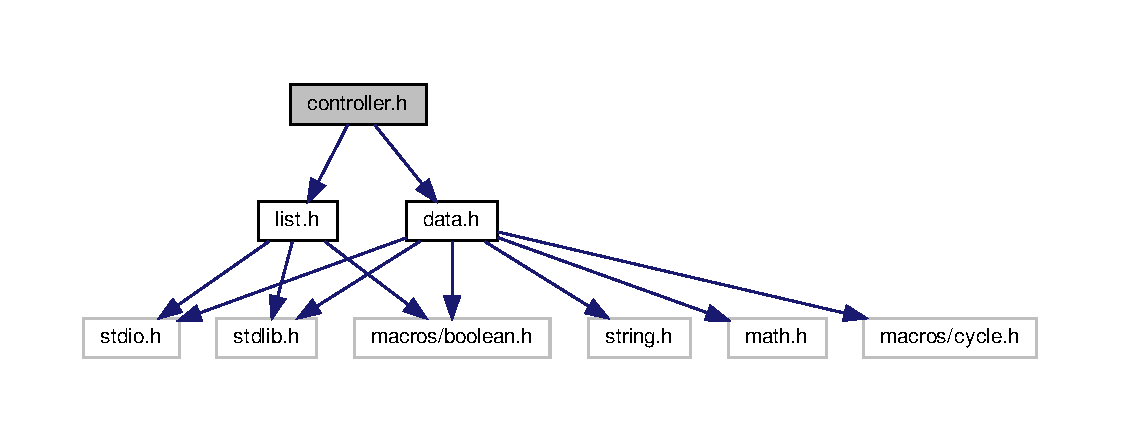
\includegraphics[width=350pt]{controller_8h__incl}
\end{center}
\end{figure}
This graph shows which files directly or indirectly include this file\+:\nopagebreak
\begin{figure}[H]
\begin{center}
\leavevmode
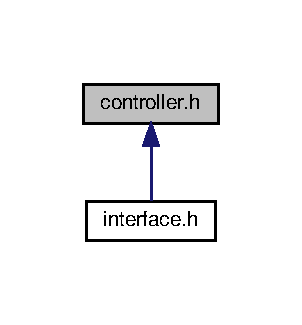
\includegraphics[width=145pt]{controller_8h__dep__incl}
\end{center}
\end{figure}
\subsection*{Functions}
\begin{DoxyCompactItemize}
\item 
\hyperlink{data_8h_ab8d2e03f1be6ed043ab77a0ea6d0c3fd}{E\+R\+R\+OS} \hyperlink{controller_8h_a40267453816c8fee2f1b6e11dacb2929}{jogar} (\hyperlink{structESTADO}{E\+S\+T\+A\+DO} $\ast$e, \hyperlink{structCOORDENADA}{C\+O\+O\+R\+D\+E\+N\+A\+DA} c)
\begin{DoxyCompactList}\small\item\em Definição da função que realiza as jogadas. Nesta função são realizadas as seguintes tarefas\+: Verifica se a coordenada introduzida é vizinha, se está vazia e se está dentro do tabuleiro. Visto isto caso seja o jogador 1 a jogar , coloca a jogada no parametro ultima jogada e troca para o jogador 2. Caso seja o jogador 2 coloca também a nova jogada na ultima jogada, troca o jogador e ainda coloca no array de jogadas. Caso a jogada não seja possível retorna 1. \end{DoxyCompactList}\item 
Boolean \hyperlink{controller_8h_ac67c4b1a7c831bdbd9e0a38ad074ea17}{is\+Terminado} (\hyperlink{structESTADO}{E\+S\+T\+A\+DO} $\ast$e)
\begin{DoxyCompactList}\small\item\em Função que determina se o Jogo está terminado. Neste sentido verifica se o algum jogador chegou a casa UM ou D\+O\+IS. Caso chegue retorna True caso contrário falso. \end{DoxyCompactList}\item 
Boolean \hyperlink{controller_8h_a08e1666ed90ac193eb2544c4fd357e25}{is\+Casa\+Vizinha} (\hyperlink{structESTADO}{E\+S\+T\+A\+DO} $\ast$e, \hyperlink{structCOORDENADA}{C\+O\+O\+R\+D\+E\+N\+A\+DA} c)
\begin{DoxyCompactList}\small\item\em Função que verifica se a jogada a ser realizada é vizinha da casa anterior. Retorna True caso seja, False caso contrário. \end{DoxyCompactList}\item 
\hyperlink{data_8h_ab8d2e03f1be6ed043ab77a0ea6d0c3fd}{E\+R\+R\+OS} \hyperlink{controller_8h_a626d31a8bad5c3f4fa84afc0c5f987ef}{gravar} (\hyperlink{structESTADO}{E\+S\+T\+A\+DO} $\ast$e, char $\ast$filename)
\begin{DoxyCompactList}\small\item\em Função que grava o tabuleiro no seu estado atual para um ficheiro de texto. \end{DoxyCompactList}\item 
\hyperlink{data_8h_ab8d2e03f1be6ed043ab77a0ea6d0c3fd}{E\+R\+R\+OS} \hyperlink{controller_8h_a6b2c21f1f942998df07e3e31c45021c9}{ler} (\hyperlink{structESTADO}{E\+S\+T\+A\+DO} $\ast$e, char $\ast$filename)
\begin{DoxyCompactList}\small\item\em Função que lê um ficheiro e converte cada linha do mesmo para uma linha de tabuleiro do Estado do jogo. \end{DoxyCompactList}\item 
int \hyperlink{controller_8h_ae7e229be0513d84bfae07481bb8461cc}{winner} (\hyperlink{structESTADO}{E\+S\+T\+A\+DO} $\ast$e)
\begin{DoxyCompactList}\small\item\em Função que determina qual foi o jogador que venceu o jogo. Avalia portanto se o jogador se encontra na casa UM ou casa D\+O\+IS ou se está rodeado. \end{DoxyCompactList}\item 
Boolean \hyperlink{controller_8h_aeef7aee77236ee9789abdc771481e83d}{go\+To\+Pos} (\hyperlink{structESTADO}{E\+S\+T\+A\+DO} $\ast$e, int n)
\begin{DoxyCompactList}\small\item\em Faz o jogo se movimentar entre jogadas podendo ir desde a jogada 0 até à ultima jogada. \end{DoxyCompactList}\end{DoxyCompactItemize}


\subsection{Detailed Description}
Definição da lógica e controlo do estado 

\subsection{Function Documentation}
\mbox{\Hypertarget{controller_8h_aeef7aee77236ee9789abdc771481e83d}\label{controller_8h_aeef7aee77236ee9789abdc771481e83d}} 
\index{controller.\+h@{controller.\+h}!go\+To\+Pos@{go\+To\+Pos}}
\index{go\+To\+Pos@{go\+To\+Pos}!controller.\+h@{controller.\+h}}
\subsubsection{\texorpdfstring{go\+To\+Pos()}{goToPos()}}
{\footnotesize\ttfamily Boolean go\+To\+Pos (\begin{DoxyParamCaption}\item[{\hyperlink{structESTADO}{E\+S\+T\+A\+DO} $\ast$}]{e,  }\item[{int}]{n }\end{DoxyParamCaption})}



Faz o jogo se movimentar entre jogadas podendo ir desde a jogada 0 até à ultima jogada. 


\begin{DoxyParams}{Parameters}
{\em e} & -\/ Estado do jogo \\
\hline
{\em n} & -\/ Jogada a partir de onde se vai continuar o jogo \\
\hline
\end{DoxyParams}
\begin{DoxyReturn}{Returns}
True caso seja possivel e False caso contrario 
\end{DoxyReturn}
\mbox{\Hypertarget{controller_8h_a626d31a8bad5c3f4fa84afc0c5f987ef}\label{controller_8h_a626d31a8bad5c3f4fa84afc0c5f987ef}} 
\index{controller.\+h@{controller.\+h}!gravar@{gravar}}
\index{gravar@{gravar}!controller.\+h@{controller.\+h}}
\subsubsection{\texorpdfstring{gravar()}{gravar()}}
{\footnotesize\ttfamily \hyperlink{data_8h_ab8d2e03f1be6ed043ab77a0ea6d0c3fd}{E\+R\+R\+OS} gravar (\begin{DoxyParamCaption}\item[{\hyperlink{structESTADO}{E\+S\+T\+A\+DO} $\ast$}]{e,  }\item[{char $\ast$}]{filename }\end{DoxyParamCaption})}



Função que grava o tabuleiro no seu estado atual para um ficheiro de texto. 


\begin{DoxyParams}{Parameters}
{\em e} & Apontador para o estado \\
\hline
{\em filename} & Nome do ficheiro que sera gravado \\
\hline
\end{DoxyParams}
\begin{DoxyReturn}{Returns}
OK no caso de ter gravado com sucesso, E\+R\+R\+O\+\_\+\+A\+B\+R\+I\+R\+\_\+\+F\+I\+C\+H\+E\+I\+RO caso contrário 
\end{DoxyReturn}
\mbox{\Hypertarget{controller_8h_a08e1666ed90ac193eb2544c4fd357e25}\label{controller_8h_a08e1666ed90ac193eb2544c4fd357e25}} 
\index{controller.\+h@{controller.\+h}!is\+Casa\+Vizinha@{is\+Casa\+Vizinha}}
\index{is\+Casa\+Vizinha@{is\+Casa\+Vizinha}!controller.\+h@{controller.\+h}}
\subsubsection{\texorpdfstring{is\+Casa\+Vizinha()}{isCasaVizinha()}}
{\footnotesize\ttfamily Boolean is\+Casa\+Vizinha (\begin{DoxyParamCaption}\item[{\hyperlink{structESTADO}{E\+S\+T\+A\+DO} $\ast$}]{e,  }\item[{\hyperlink{structCOORDENADA}{C\+O\+O\+R\+D\+E\+N\+A\+DA}}]{c }\end{DoxyParamCaption})}



Função que verifica se a jogada a ser realizada é vizinha da casa anterior. Retorna True caso seja, False caso contrário. 


\begin{DoxyParams}{Parameters}
{\em e} & Apontador para o estado \\
\hline
{\em c} & Coordanada da casa atual \\
\hline
\end{DoxyParams}
\begin{DoxyReturn}{Returns}
True no caso de c ser vizinha da posição atual, False caso contrário 
\end{DoxyReturn}
\mbox{\Hypertarget{controller_8h_ac67c4b1a7c831bdbd9e0a38ad074ea17}\label{controller_8h_ac67c4b1a7c831bdbd9e0a38ad074ea17}} 
\index{controller.\+h@{controller.\+h}!is\+Terminado@{is\+Terminado}}
\index{is\+Terminado@{is\+Terminado}!controller.\+h@{controller.\+h}}
\subsubsection{\texorpdfstring{is\+Terminado()}{isTerminado()}}
{\footnotesize\ttfamily Boolean is\+Terminado (\begin{DoxyParamCaption}\item[{\hyperlink{structESTADO}{E\+S\+T\+A\+DO} $\ast$}]{e }\end{DoxyParamCaption})}



Função que determina se o Jogo está terminado. Neste sentido verifica se o algum jogador chegou a casa UM ou D\+O\+IS. Caso chegue retorna True caso contrário falso. 


\begin{DoxyParams}{Parameters}
{\em e} & Apontador para o estado \\
\hline
\end{DoxyParams}
\begin{DoxyReturn}{Returns}
True no caso de o jogo ter terminado, False caso contrário 
\end{DoxyReturn}
\mbox{\Hypertarget{controller_8h_a40267453816c8fee2f1b6e11dacb2929}\label{controller_8h_a40267453816c8fee2f1b6e11dacb2929}} 
\index{controller.\+h@{controller.\+h}!jogar@{jogar}}
\index{jogar@{jogar}!controller.\+h@{controller.\+h}}
\subsubsection{\texorpdfstring{jogar()}{jogar()}}
{\footnotesize\ttfamily \hyperlink{data_8h_ab8d2e03f1be6ed043ab77a0ea6d0c3fd}{E\+R\+R\+OS} jogar (\begin{DoxyParamCaption}\item[{\hyperlink{structESTADO}{E\+S\+T\+A\+DO} $\ast$}]{e,  }\item[{\hyperlink{structCOORDENADA}{C\+O\+O\+R\+D\+E\+N\+A\+DA}}]{c }\end{DoxyParamCaption})}



Definição da função que realiza as jogadas. Nesta função são realizadas as seguintes tarefas\+: Verifica se a coordenada introduzida é vizinha, se está vazia e se está dentro do tabuleiro. Visto isto caso seja o jogador 1 a jogar , coloca a jogada no parametro ultima jogada e troca para o jogador 2. Caso seja o jogador 2 coloca também a nova jogada na ultima jogada, troca o jogador e ainda coloca no array de jogadas. Caso a jogada não seja possível retorna 1. 


\begin{DoxyParams}{Parameters}
{\em estado} & Apontador para o estado \\
\hline
{\em c} & A coordenada \\
\hline
\end{DoxyParams}
\begin{DoxyReturn}{Returns}
1 no caso de a jogada ser válida e 0 no caso contrário 
\end{DoxyReturn}
\mbox{\Hypertarget{controller_8h_a6b2c21f1f942998df07e3e31c45021c9}\label{controller_8h_a6b2c21f1f942998df07e3e31c45021c9}} 
\index{controller.\+h@{controller.\+h}!ler@{ler}}
\index{ler@{ler}!controller.\+h@{controller.\+h}}
\subsubsection{\texorpdfstring{ler()}{ler()}}
{\footnotesize\ttfamily \hyperlink{data_8h_ab8d2e03f1be6ed043ab77a0ea6d0c3fd}{E\+R\+R\+OS} ler (\begin{DoxyParamCaption}\item[{\hyperlink{structESTADO}{E\+S\+T\+A\+DO} $\ast$}]{e,  }\item[{char $\ast$}]{filename }\end{DoxyParamCaption})}



Função que lê um ficheiro e converte cada linha do mesmo para uma linha de tabuleiro do Estado do jogo. 


\begin{DoxyParams}{Parameters}
{\em e} & Apontador para o estado \\
\hline
{\em filename} & Nome do ficheiro para ler \\
\hline
\end{DoxyParams}
\begin{DoxyReturn}{Returns}
OK no caso de ter gravado com sucesso, E\+R\+R\+O\+\_\+\+A\+B\+R\+I\+R\+\_\+\+F\+I\+C\+H\+E\+I\+RO caso contrário 
\end{DoxyReturn}
\mbox{\Hypertarget{controller_8h_ae7e229be0513d84bfae07481bb8461cc}\label{controller_8h_ae7e229be0513d84bfae07481bb8461cc}} 
\index{controller.\+h@{controller.\+h}!winner@{winner}}
\index{winner@{winner}!controller.\+h@{controller.\+h}}
\subsubsection{\texorpdfstring{winner()}{winner()}}
{\footnotesize\ttfamily int winner (\begin{DoxyParamCaption}\item[{\hyperlink{structESTADO}{E\+S\+T\+A\+DO} $\ast$}]{e }\end{DoxyParamCaption})}



Função que determina qual foi o jogador que venceu o jogo. Avalia portanto se o jogador se encontra na casa UM ou casa D\+O\+IS ou se está rodeado. 


\begin{DoxyParams}{Parameters}
{\em e} & Apontador para o estado \\
\hline
\end{DoxyParams}
\begin{DoxyReturn}{Returns}
O jogador vencedor 
\end{DoxyReturn}

\hypertarget{data_8h}{}\section{data.\+h File Reference}
\label{data_8h}\index{data.\+h@{data.\+h}}
{\ttfamily \#include $<$stdio.\+h$>$}\newline
{\ttfamily \#include $<$stdlib.\+h$>$}\newline
{\ttfamily \#include $<$string.\+h$>$}\newline
{\ttfamily \#include $<$math.\+h$>$}\newline
{\ttfamily \#include \char`\"{}macros/cycle.\+h\char`\"{}}\newline
{\ttfamily \#include \char`\"{}macros/boolean.\+h\char`\"{}}\newline
Include dependency graph for data.\+h\+:
\nopagebreak
\begin{figure}[H]
\begin{center}
\leavevmode
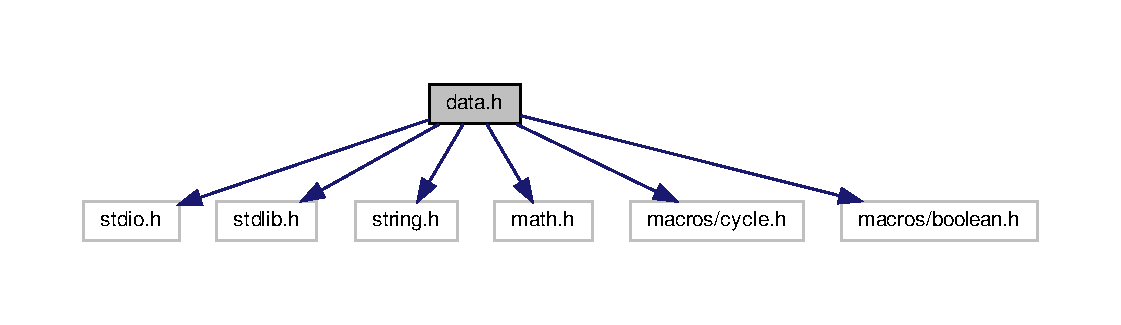
\includegraphics[width=350pt]{data_8h__incl}
\end{center}
\end{figure}
This graph shows which files directly or indirectly include this file\+:
\nopagebreak
\begin{figure}[H]
\begin{center}
\leavevmode
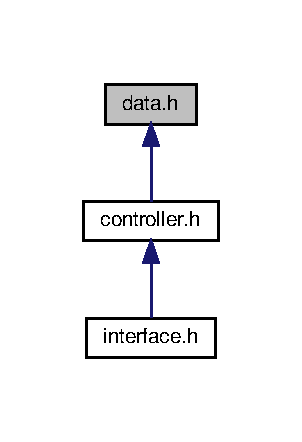
\includegraphics[width=145pt]{data_8h__dep__incl}
\end{center}
\end{figure}
\subsection*{Classes}
\begin{DoxyCompactItemize}
\item 
struct \hyperlink{structCOORDENADA}{C\+O\+O\+R\+D\+E\+N\+A\+DA}
\begin{DoxyCompactList}\small\item\em Tipo de dados para as coordenadas. \end{DoxyCompactList}\item 
struct \hyperlink{structJOGADA}{J\+O\+G\+A\+DA}
\begin{DoxyCompactList}\small\item\em Tipo de dados para a jogada. \end{DoxyCompactList}\item 
struct \hyperlink{structESTADO}{E\+S\+T\+A\+DO}
\begin{DoxyCompactList}\small\item\em Tipo de dados para o estado. \end{DoxyCompactList}\end{DoxyCompactItemize}
\subsection*{Typedefs}
\begin{DoxyCompactItemize}
\item 
\mbox{\Hypertarget{data_8h_a94c221d29a1760f008b7834093259b7d}\label{data_8h_a94c221d29a1760f008b7834093259b7d}} 
typedef \hyperlink{structJOGADA}{J\+O\+G\+A\+DA} \hyperlink{data_8h_a94c221d29a1760f008b7834093259b7d}{J\+O\+G\+A\+D\+AS}\mbox{[}32\mbox{]}
\begin{DoxyCompactList}\small\item\em Tipo de dados para as jogadas. \end{DoxyCompactList}\end{DoxyCompactItemize}
\subsection*{Enumerations}
\begin{DoxyCompactItemize}
\item 
\mbox{\Hypertarget{data_8h_ab8d2e03f1be6ed043ab77a0ea6d0c3fd}\label{data_8h_ab8d2e03f1be6ed043ab77a0ea6d0c3fd}} 
enum \hyperlink{data_8h_ab8d2e03f1be6ed043ab77a0ea6d0c3fd}{E\+R\+R\+OS} \{ \newline
{\bfseries OK}, 
{\bfseries C\+O\+O\+R\+D\+E\+N\+A\+D\+A\+\_\+\+I\+N\+V\+A\+L\+I\+DA}, 
{\bfseries J\+O\+G\+A\+D\+A\+\_\+\+I\+N\+V\+A\+L\+I\+DA}, 
{\bfseries E\+R\+R\+O\+\_\+\+L\+E\+R\+\_\+\+T\+AB}, 
\newline
{\bfseries E\+R\+R\+O\+\_\+\+A\+B\+R\+I\+R\+\_\+\+F\+I\+C\+H\+E\+I\+RO}
 \}\begin{DoxyCompactList}\small\item\em Tipo de dados para os erros. \end{DoxyCompactList}
\item 
\mbox{\Hypertarget{data_8h_aba91601f16d4c485b2d9b8c429f27039}\label{data_8h_aba91601f16d4c485b2d9b8c429f27039}} 
enum \hyperlink{data_8h_aba91601f16d4c485b2d9b8c429f27039}{C\+A\+SA} \{ \newline
{\bfseries UM} = \textquotesingle{}1\textquotesingle{}, 
{\bfseries D\+O\+IS} = \textquotesingle{}2\textquotesingle{}, 
{\bfseries V\+A\+Z\+IO} = \textquotesingle{}.\textquotesingle{}, 
{\bfseries B\+R\+A\+N\+CA} = \textquotesingle{}$\ast$\textquotesingle{}, 
\newline
{\bfseries P\+R\+E\+TA} = \textquotesingle{}\#\textquotesingle{}
 \}\begin{DoxyCompactList}\small\item\em Tipo de dados para a casa. \end{DoxyCompactList}
\end{DoxyCompactItemize}
\subsection*{Functions}
\begin{DoxyCompactItemize}
\item 
int \hyperlink{data_8h_aa6737cfda62eb8368073d1457962ea36}{get\+Pointer\+Jogada} (\hyperlink{structESTADO}{E\+S\+T\+A\+DO} $\ast$e)
\begin{DoxyCompactList}\small\item\em Função usada para obter o pointer da posiçao do estado no array de jogadas. \end{DoxyCompactList}\item 
void \hyperlink{data_8h_a32b3e19b6762b1ab390a7b37058bcac4}{set\+Pointer\+Jogada} (\hyperlink{structESTADO}{E\+S\+T\+A\+DO} $\ast$e, int num)
\begin{DoxyCompactList}\small\item\em Altera o valor do pointer que indica a jogada atual. \end{DoxyCompactList}\item 
void \hyperlink{data_8h_aa2205e147ba0ada94666920611ebdd3f}{renicializa\+Tab} (\hyperlink{structESTADO}{E\+S\+T\+A\+DO} $\ast$e)
\begin{DoxyCompactList}\small\item\em Retorna o tabuleiro para o seu valor inicial. \end{DoxyCompactList}\item 
void \hyperlink{data_8h_a9d58c94323f44719b333380934c1a57c}{inc\+Pointer\+Jogada} (\hyperlink{structESTADO}{E\+S\+T\+A\+DO} $\ast$e)
\begin{DoxyCompactList}\small\item\em Incrementa o pointer da posicao do estado no array. \end{DoxyCompactList}\item 
\hyperlink{structCOORDENADA}{C\+O\+O\+R\+D\+E\+N\+A\+DA} \hyperlink{data_8h_a1999bafee85ae84698b9c2db31b1ba99}{set\+Coordenada} (int line, int col)
\begin{DoxyCompactList}\small\item\em Função que cria uma coordenada as coordenadas respetivas para a coluna e linha. \end{DoxyCompactList}\item 
int \hyperlink{data_8h_a0183a44bde7867f6c417e584afa8e56e}{get\+Coluna} (\hyperlink{structCOORDENADA}{C\+O\+O\+R\+D\+E\+N\+A\+DA} c)
\begin{DoxyCompactList}\small\item\em Função que dada um coordenada devolve o parâmetro da coluna. \end{DoxyCompactList}\item 
int \hyperlink{data_8h_a79cea1ec53fca591b4803ac0393bdaee}{get\+Linha} (\hyperlink{structCOORDENADA}{C\+O\+O\+R\+D\+E\+N\+A\+DA} c)
\begin{DoxyCompactList}\small\item\em Função que dada um coordenada devolve o parâmetro da linha. \end{DoxyCompactList}\item 
\hyperlink{structCOORDENADA}{C\+O\+O\+R\+D\+E\+N\+A\+DA} \hyperlink{data_8h_ab4332447f942e9a8268ccce3e0d5854c}{create\+Null\+Coord} ()
\begin{DoxyCompactList}\small\item\em Funcao que cria uma coordenada Nula Serve maioritariamente para o caso de criar uma jogada mas sem o jogador 2 ter ainda jogado. \end{DoxyCompactList}\item 
Boolean \hyperlink{data_8h_ae1315370ef7e22e1cbd289d8a08b99b2}{is\+Null\+Coord} (\hyperlink{structCOORDENADA}{C\+O\+O\+R\+D\+E\+N\+A\+DA} c)
\begin{DoxyCompactList}\small\item\em Verifica se uma coordenada é null. \end{DoxyCompactList}\item 
\hyperlink{data_8h_aba91601f16d4c485b2d9b8c429f27039}{C\+A\+SA} \hyperlink{data_8h_acb8160cac1e3533d3e0c268f0a65bf36}{get\+Casa\+\_\+ultima\+Jogada} (\hyperlink{structESTADO}{E\+S\+T\+A\+DO} $\ast$e)
\begin{DoxyCompactList}\small\item\em Função que devolve a casa onde a ultima casa foi realizada. \end{DoxyCompactList}\item 
\hyperlink{structCOORDENADA}{C\+O\+O\+R\+D\+E\+N\+A\+DA} \hyperlink{data_8h_a2d1d1300cb689bfade0c8ab736a5c2ed}{get\+Coordenada} (\hyperlink{structJOGADA}{J\+O\+G\+A\+DA} j, int jogador)
\begin{DoxyCompactList}\small\item\em Função que devolve a coordenada de uma jogada, ou seja, a coordenada do jogador 1 ou jogador 2. \end{DoxyCompactList}\item 
\hyperlink{structJOGADA}{J\+O\+G\+A\+DA} \hyperlink{data_8h_a3697cf4d8e8eeafdc4e31dbdfd6c45bb}{create\+Jogada} (\hyperlink{structCOORDENADA}{C\+O\+O\+R\+D\+E\+N\+A\+DA} c1, \hyperlink{structCOORDENADA}{C\+O\+O\+R\+D\+E\+N\+A\+DA} c2)
\begin{DoxyCompactList}\small\item\em Função que dada duas coordenadas cria uma \hyperlink{structJOGADA}{J\+O\+G\+A\+DA} e retorna a respetiva jogada. \end{DoxyCompactList}\item 
\hyperlink{structJOGADA}{J\+O\+G\+A\+DA} \hyperlink{data_8h_a252b653cecd65225969ef0fbc457d226}{get\+Jogada} (\hyperlink{structESTADO}{E\+S\+T\+A\+DO} $\ast$e, int idx)
\begin{DoxyCompactList}\small\item\em Função que recebe uma jogada num determinado indice. \end{DoxyCompactList}\item 
\hyperlink{structCOORDENADA}{C\+O\+O\+R\+D\+E\+N\+A\+DA} \hyperlink{data_8h_a8d7adf2965f060b0834e87e1aed7e209}{get\+Ultima\+Jogada} (\hyperlink{structESTADO}{E\+S\+T\+A\+DO} $\ast$e)
\begin{DoxyCompactList}\small\item\em Função que obtém a ultima jogada realizada. \end{DoxyCompactList}\item 
void \hyperlink{data_8h_a261951f5a3b69e5ffa6edb742f7fd5e8}{set\+Ultima\+Jogada} (\hyperlink{structESTADO}{E\+S\+T\+A\+DO} $\ast$e, \hyperlink{structCOORDENADA}{C\+O\+O\+R\+D\+E\+N\+A\+DA} c1)
\begin{DoxyCompactList}\small\item\em Função que coloca a ultima jogada no estado. \end{DoxyCompactList}\item 
void \hyperlink{data_8h_a5156aa8d30673f3bd7b1190fd04103de}{add\+To\+Jogadas} (\hyperlink{structESTADO}{E\+S\+T\+A\+DO} $\ast$e, \hyperlink{structJOGADA}{J\+O\+G\+A\+DA} j)
\begin{DoxyCompactList}\small\item\em Função que adiciona um \hyperlink{structJOGADA}{J\+O\+G\+A\+DA} j ao estado. \end{DoxyCompactList}\item 
void \hyperlink{data_8h_ae893525430d4ceb49841b95443a96728}{edit\+Jogadas} (\hyperlink{structESTADO}{E\+S\+T\+A\+DO} $\ast$e, \hyperlink{structJOGADA}{J\+O\+G\+A\+DA} j, int idx)
\begin{DoxyCompactList}\small\item\em Troca a jogada num dado indice por outra. \end{DoxyCompactList}\item 
int \hyperlink{data_8h_a12874adb19d5d154a3af0f3028d17d3b}{get\+Num\+Jogadas} (\hyperlink{structESTADO}{E\+S\+T\+A\+DO} $\ast$e)
\begin{DoxyCompactList}\small\item\em Função que retorna o numero de jogadas. \end{DoxyCompactList}\item 
void \hyperlink{data_8h_afb2751df87d43bd3a78dccb7c6aa0cc0}{set\+Num\+Jogadas} (\hyperlink{structESTADO}{E\+S\+T\+A\+DO} $\ast$e, int num)
\begin{DoxyCompactList}\small\item\em Altera o numero de jogadas atual para um dado numero. \end{DoxyCompactList}\item 
void \hyperlink{data_8h_a9aceecbb9febd75affa41ed245740268}{inc\+Num\+Jogadas} (\hyperlink{structESTADO}{E\+S\+T\+A\+DO} $\ast$e)
\begin{DoxyCompactList}\small\item\em Função que incrementa o numero de jogadas. \end{DoxyCompactList}\item 
\hyperlink{data_8h_aba91601f16d4c485b2d9b8c429f27039}{C\+A\+SA} \hyperlink{data_8h_a91f22f1ec4a44d41ae7dbcc449157d47}{get\+Casa} (\hyperlink{structESTADO}{E\+S\+T\+A\+DO} $\ast$e, \hyperlink{structCOORDENADA}{C\+O\+O\+R\+D\+E\+N\+A\+DA} c)
\begin{DoxyCompactList}\small\item\em Função que acede ao estado e ve qual a casa que se encontra numa determinada coordenada c. \end{DoxyCompactList}\item 
void \hyperlink{data_8h_a6f0eddb6649f61e6fa2293252f6dd749}{set\+Casa} (\hyperlink{structESTADO}{E\+S\+T\+A\+DO} $\ast$e, \hyperlink{structCOORDENADA}{C\+O\+O\+R\+D\+E\+N\+A\+DA} c, \hyperlink{data_8h_aba91601f16d4c485b2d9b8c429f27039}{C\+A\+SA} casa)
\begin{DoxyCompactList}\small\item\em Função que coloca uma casa numa determinada coordenada no estado. \end{DoxyCompactList}\item 
\hyperlink{data_8h_aba91601f16d4c485b2d9b8c429f27039}{C\+A\+SA} \hyperlink{data_8h_af257fae5e735a17794b8c906b6b4d563}{get\+Casa\+\_\+parametro} (\hyperlink{structESTADO}{E\+S\+T\+A\+DO} $\ast$e, int x, int y)
\begin{DoxyCompactList}\small\item\em Função que recebe coordenadas de dois inteiros e encontra a respetiva casa no estado. \end{DoxyCompactList}\item 
void \hyperlink{data_8h_a7ad8db36a0e0e59670e1bc940fe6b09d}{swap\+Jogador} (\hyperlink{structESTADO}{E\+S\+T\+A\+DO} $\ast$e)
\begin{DoxyCompactList}\small\item\em Função que acede ao estado e muda o jogador, caso seja 1 muda para 2 e vice-\/versa. \end{DoxyCompactList}\item 
void \hyperlink{data_8h_a7ecad922782940ee6ed0f40106330c63}{set\+Jogador} (\hyperlink{structESTADO}{E\+S\+T\+A\+DO} $\ast$e, int jogador)
\begin{DoxyCompactList}\small\item\em Funcao que altera o jogador atual. \end{DoxyCompactList}\item 
int \hyperlink{data_8h_a10993347e610b194752a0afda93e2d47}{getjogador} (\hyperlink{structESTADO}{E\+S\+T\+A\+DO} $\ast$e)
\begin{DoxyCompactList}\small\item\em Função que retorna qual é o jogador que está a jogar atual. \end{DoxyCompactList}\item 
void \hyperlink{data_8h_abbe3b034f746515b4d678e3526c8d97d}{reset\+Estado} (\hyperlink{structESTADO}{E\+S\+T\+A\+DO} $\ast$e)
\begin{DoxyCompactList}\small\item\em Retorna alguns valores do estado para o inicial. \end{DoxyCompactList}\item 
\hyperlink{structESTADO}{E\+S\+T\+A\+DO} $\ast$ \hyperlink{data_8h_a7e0c7e26fb685d9ab501e19b05e6954f}{inicializar\+\_\+estado} ()
\begin{DoxyCompactList}\small\item\em Inicializa o estado do jogo A peça branca começa na coluna 4 da linha 4 e considera se essa a ultima jogada Todo o resto do tabuleiro é inicializado a V\+A\+Z\+IO O tabuleiro é representado por um array bidimensional do tipo tab\mbox{[}linha\mbox{]}\mbox{[}coluna\mbox{]}. \end{DoxyCompactList}\end{DoxyCompactItemize}


\subsection{Detailed Description}
Definição do estado e das funções que o manipulam 

\subsection{Function Documentation}
\mbox{\Hypertarget{data_8h_a5156aa8d30673f3bd7b1190fd04103de}\label{data_8h_a5156aa8d30673f3bd7b1190fd04103de}} 
\index{data.\+h@{data.\+h}!add\+To\+Jogadas@{add\+To\+Jogadas}}
\index{add\+To\+Jogadas@{add\+To\+Jogadas}!data.\+h@{data.\+h}}
\subsubsection{\texorpdfstring{add\+To\+Jogadas()}{addToJogadas()}}
{\footnotesize\ttfamily void add\+To\+Jogadas (\begin{DoxyParamCaption}\item[{\hyperlink{structESTADO}{E\+S\+T\+A\+DO} $\ast$}]{e,  }\item[{\hyperlink{structJOGADA}{J\+O\+G\+A\+DA}}]{j }\end{DoxyParamCaption})}



Função que adiciona um \hyperlink{structJOGADA}{J\+O\+G\+A\+DA} j ao estado. 


\begin{DoxyParams}{Parameters}
{\em e} & -\/ Estado do jogo \\
\hline
{\em j} & -\/ Jogada a ser adicionada \\
\hline
\end{DoxyParams}
\mbox{\Hypertarget{data_8h_a3697cf4d8e8eeafdc4e31dbdfd6c45bb}\label{data_8h_a3697cf4d8e8eeafdc4e31dbdfd6c45bb}} 
\index{data.\+h@{data.\+h}!create\+Jogada@{create\+Jogada}}
\index{create\+Jogada@{create\+Jogada}!data.\+h@{data.\+h}}
\subsubsection{\texorpdfstring{create\+Jogada()}{createJogada()}}
{\footnotesize\ttfamily \hyperlink{structJOGADA}{J\+O\+G\+A\+DA} create\+Jogada (\begin{DoxyParamCaption}\item[{\hyperlink{structCOORDENADA}{C\+O\+O\+R\+D\+E\+N\+A\+DA}}]{c1,  }\item[{\hyperlink{structCOORDENADA}{C\+O\+O\+R\+D\+E\+N\+A\+DA}}]{c2 }\end{DoxyParamCaption})}



Função que dada duas coordenadas cria uma \hyperlink{structJOGADA}{J\+O\+G\+A\+DA} e retorna a respetiva jogada. 


\begin{DoxyParams}{Parameters}
{\em c1} & -\/ Primeira coordenada \\
\hline
{\em c2} & -\/ Segunda coordenada \\
\hline
\end{DoxyParams}
\begin{DoxyReturn}{Returns}
\hyperlink{structJOGADA}{J\+O\+G\+A\+DA} adicionada 
\end{DoxyReturn}
\mbox{\Hypertarget{data_8h_ab4332447f942e9a8268ccce3e0d5854c}\label{data_8h_ab4332447f942e9a8268ccce3e0d5854c}} 
\index{data.\+h@{data.\+h}!create\+Null\+Coord@{create\+Null\+Coord}}
\index{create\+Null\+Coord@{create\+Null\+Coord}!data.\+h@{data.\+h}}
\subsubsection{\texorpdfstring{create\+Null\+Coord()}{createNullCoord()}}
{\footnotesize\ttfamily \hyperlink{structCOORDENADA}{C\+O\+O\+R\+D\+E\+N\+A\+DA} create\+Null\+Coord (\begin{DoxyParamCaption}{ }\end{DoxyParamCaption})}



Funcao que cria uma coordenada Nula Serve maioritariamente para o caso de criar uma jogada mas sem o jogador 2 ter ainda jogado. 

\begin{DoxyReturn}{Returns}
Uma coordenada onde a coluna e a linha são -\/1 
\end{DoxyReturn}
\mbox{\Hypertarget{data_8h_ae893525430d4ceb49841b95443a96728}\label{data_8h_ae893525430d4ceb49841b95443a96728}} 
\index{data.\+h@{data.\+h}!edit\+Jogadas@{edit\+Jogadas}}
\index{edit\+Jogadas@{edit\+Jogadas}!data.\+h@{data.\+h}}
\subsubsection{\texorpdfstring{edit\+Jogadas()}{editJogadas()}}
{\footnotesize\ttfamily void edit\+Jogadas (\begin{DoxyParamCaption}\item[{\hyperlink{structESTADO}{E\+S\+T\+A\+DO} $\ast$}]{e,  }\item[{\hyperlink{structJOGADA}{J\+O\+G\+A\+DA}}]{j,  }\item[{int}]{idx }\end{DoxyParamCaption})}



Troca a jogada num dado indice por outra. 


\begin{DoxyParams}{Parameters}
{\em e} & Estado do jogo \\
\hline
{\em j} & Nova jogada que irá tomar o lugar da antiga \\
\hline
{\em idx} & Indice da jogada que sera para trocar \\
\hline
\end{DoxyParams}
\mbox{\Hypertarget{data_8h_a91f22f1ec4a44d41ae7dbcc449157d47}\label{data_8h_a91f22f1ec4a44d41ae7dbcc449157d47}} 
\index{data.\+h@{data.\+h}!get\+Casa@{get\+Casa}}
\index{get\+Casa@{get\+Casa}!data.\+h@{data.\+h}}
\subsubsection{\texorpdfstring{get\+Casa()}{getCasa()}}
{\footnotesize\ttfamily \hyperlink{data_8h_aba91601f16d4c485b2d9b8c429f27039}{C\+A\+SA} get\+Casa (\begin{DoxyParamCaption}\item[{\hyperlink{structESTADO}{E\+S\+T\+A\+DO} $\ast$}]{e,  }\item[{\hyperlink{structCOORDENADA}{C\+O\+O\+R\+D\+E\+N\+A\+DA}}]{c }\end{DoxyParamCaption})}



Função que acede ao estado e ve qual a casa que se encontra numa determinada coordenada c. 


\begin{DoxyParams}{Parameters}
{\em e} & -\/ Estado do jogo \\
\hline
{\em c} & -\/ Coordenada a procurar \\
\hline
\end{DoxyParams}
\begin{DoxyReturn}{Returns}
Casa que está na respetiva coordenada 
\end{DoxyReturn}
\mbox{\Hypertarget{data_8h_af257fae5e735a17794b8c906b6b4d563}\label{data_8h_af257fae5e735a17794b8c906b6b4d563}} 
\index{data.\+h@{data.\+h}!get\+Casa\+\_\+parametro@{get\+Casa\+\_\+parametro}}
\index{get\+Casa\+\_\+parametro@{get\+Casa\+\_\+parametro}!data.\+h@{data.\+h}}
\subsubsection{\texorpdfstring{get\+Casa\+\_\+parametro()}{getCasa\_parametro()}}
{\footnotesize\ttfamily \hyperlink{data_8h_aba91601f16d4c485b2d9b8c429f27039}{C\+A\+SA} get\+Casa\+\_\+parametro (\begin{DoxyParamCaption}\item[{\hyperlink{structESTADO}{E\+S\+T\+A\+DO} $\ast$}]{e,  }\item[{int}]{x,  }\item[{int}]{y }\end{DoxyParamCaption})}



Função que recebe coordenadas de dois inteiros e encontra a respetiva casa no estado. 


\begin{DoxyParams}{Parameters}
{\em e} & -\/ Estado inicial do jogo \\
\hline
{\em x} & -\/ Parametro da linha \\
\hline
{\em y} & -\/ Parâmetro da coluna \\
\hline
\end{DoxyParams}
\begin{DoxyReturn}{Returns}
Casa que se encontra em x e y 
\end{DoxyReturn}
\mbox{\Hypertarget{data_8h_acb8160cac1e3533d3e0c268f0a65bf36}\label{data_8h_acb8160cac1e3533d3e0c268f0a65bf36}} 
\index{data.\+h@{data.\+h}!get\+Casa\+\_\+ultima\+Jogada@{get\+Casa\+\_\+ultima\+Jogada}}
\index{get\+Casa\+\_\+ultima\+Jogada@{get\+Casa\+\_\+ultima\+Jogada}!data.\+h@{data.\+h}}
\subsubsection{\texorpdfstring{get\+Casa\+\_\+ultima\+Jogada()}{getCasa\_ultimaJogada()}}
{\footnotesize\ttfamily \hyperlink{data_8h_aba91601f16d4c485b2d9b8c429f27039}{C\+A\+SA} get\+Casa\+\_\+ultima\+Jogada (\begin{DoxyParamCaption}\item[{\hyperlink{structESTADO}{E\+S\+T\+A\+DO} $\ast$}]{e }\end{DoxyParamCaption})}



Função que devolve a casa onde a ultima casa foi realizada. 


\begin{DoxyParams}{Parameters}
{\em e} & -\/ Estado do jogo. \\
\hline
\end{DoxyParams}
\begin{DoxyReturn}{Returns}
Casa 
\end{DoxyReturn}
\mbox{\Hypertarget{data_8h_a0183a44bde7867f6c417e584afa8e56e}\label{data_8h_a0183a44bde7867f6c417e584afa8e56e}} 
\index{data.\+h@{data.\+h}!get\+Coluna@{get\+Coluna}}
\index{get\+Coluna@{get\+Coluna}!data.\+h@{data.\+h}}
\subsubsection{\texorpdfstring{get\+Coluna()}{getColuna()}}
{\footnotesize\ttfamily int get\+Coluna (\begin{DoxyParamCaption}\item[{\hyperlink{structCOORDENADA}{C\+O\+O\+R\+D\+E\+N\+A\+DA}}]{c }\end{DoxyParamCaption})}



Função que dada um coordenada devolve o parâmetro da coluna. 


\begin{DoxyParams}{Parameters}
{\em c} & -\/coordenada necessária \\
\hline
\end{DoxyParams}
\begin{DoxyReturn}{Returns}
Parâmetro da coluna 
\end{DoxyReturn}
\mbox{\Hypertarget{data_8h_a2d1d1300cb689bfade0c8ab736a5c2ed}\label{data_8h_a2d1d1300cb689bfade0c8ab736a5c2ed}} 
\index{data.\+h@{data.\+h}!get\+Coordenada@{get\+Coordenada}}
\index{get\+Coordenada@{get\+Coordenada}!data.\+h@{data.\+h}}
\subsubsection{\texorpdfstring{get\+Coordenada()}{getCoordenada()}}
{\footnotesize\ttfamily \hyperlink{structCOORDENADA}{C\+O\+O\+R\+D\+E\+N\+A\+DA} get\+Coordenada (\begin{DoxyParamCaption}\item[{\hyperlink{structJOGADA}{J\+O\+G\+A\+DA}}]{j,  }\item[{int}]{jogador }\end{DoxyParamCaption})}



Função que devolve a coordenada de uma jogada, ou seja, a coordenada do jogador 1 ou jogador 2. 


\begin{DoxyParams}{Parameters}
{\em j} & -\/ jogada a ser analisada. \\
\hline
{\em jogador} & -\/ qual o jogador que se pretende obter a respetiva coordenada da jogada \\
\hline
\end{DoxyParams}
\begin{DoxyReturn}{Returns}
Casa 
\end{DoxyReturn}
\mbox{\Hypertarget{data_8h_a252b653cecd65225969ef0fbc457d226}\label{data_8h_a252b653cecd65225969ef0fbc457d226}} 
\index{data.\+h@{data.\+h}!get\+Jogada@{get\+Jogada}}
\index{get\+Jogada@{get\+Jogada}!data.\+h@{data.\+h}}
\subsubsection{\texorpdfstring{get\+Jogada()}{getJogada()}}
{\footnotesize\ttfamily \hyperlink{structJOGADA}{J\+O\+G\+A\+DA} get\+Jogada (\begin{DoxyParamCaption}\item[{\hyperlink{structESTADO}{E\+S\+T\+A\+DO} $\ast$}]{e,  }\item[{int}]{idx }\end{DoxyParamCaption})}



Função que recebe uma jogada num determinado indice. 


\begin{DoxyParams}{Parameters}
{\em e} & -\/ Estado do jogo \\
\hline
{\em idx} & -\/ Indice da jogada no array de jogadas \\
\hline
\end{DoxyParams}
\begin{DoxyReturn}{Returns}
Jogada obtida 
\end{DoxyReturn}
\mbox{\Hypertarget{data_8h_a10993347e610b194752a0afda93e2d47}\label{data_8h_a10993347e610b194752a0afda93e2d47}} 
\index{data.\+h@{data.\+h}!getjogador@{getjogador}}
\index{getjogador@{getjogador}!data.\+h@{data.\+h}}
\subsubsection{\texorpdfstring{getjogador()}{getjogador()}}
{\footnotesize\ttfamily int getjogador (\begin{DoxyParamCaption}\item[{\hyperlink{structESTADO}{E\+S\+T\+A\+DO} $\ast$}]{e }\end{DoxyParamCaption})}



Função que retorna qual é o jogador que está a jogar atual. 


\begin{DoxyParams}{Parameters}
{\em e} & -\/ Estado inicial \\
\hline
\end{DoxyParams}
\begin{DoxyReturn}{Returns}
Jogador atual 
\end{DoxyReturn}
\mbox{\Hypertarget{data_8h_a79cea1ec53fca591b4803ac0393bdaee}\label{data_8h_a79cea1ec53fca591b4803ac0393bdaee}} 
\index{data.\+h@{data.\+h}!get\+Linha@{get\+Linha}}
\index{get\+Linha@{get\+Linha}!data.\+h@{data.\+h}}
\subsubsection{\texorpdfstring{get\+Linha()}{getLinha()}}
{\footnotesize\ttfamily int get\+Linha (\begin{DoxyParamCaption}\item[{\hyperlink{structCOORDENADA}{C\+O\+O\+R\+D\+E\+N\+A\+DA}}]{c }\end{DoxyParamCaption})}



Função que dada um coordenada devolve o parâmetro da linha. 


\begin{DoxyParams}{Parameters}
{\em c} & -\/ coordenada necessária \\
\hline
\end{DoxyParams}
\begin{DoxyReturn}{Returns}
Parâmetro da linha 
\end{DoxyReturn}
\mbox{\Hypertarget{data_8h_a12874adb19d5d154a3af0f3028d17d3b}\label{data_8h_a12874adb19d5d154a3af0f3028d17d3b}} 
\index{data.\+h@{data.\+h}!get\+Num\+Jogadas@{get\+Num\+Jogadas}}
\index{get\+Num\+Jogadas@{get\+Num\+Jogadas}!data.\+h@{data.\+h}}
\subsubsection{\texorpdfstring{get\+Num\+Jogadas()}{getNumJogadas()}}
{\footnotesize\ttfamily int get\+Num\+Jogadas (\begin{DoxyParamCaption}\item[{\hyperlink{structESTADO}{E\+S\+T\+A\+DO} $\ast$}]{e }\end{DoxyParamCaption})}



Função que retorna o numero de jogadas. 


\begin{DoxyParams}{Parameters}
{\em e} & -\/ Estado do jogo \\
\hline
\end{DoxyParams}
\begin{DoxyReturn}{Returns}
numero de jogadas realizadas até ao momento 
\end{DoxyReturn}
\mbox{\Hypertarget{data_8h_aa6737cfda62eb8368073d1457962ea36}\label{data_8h_aa6737cfda62eb8368073d1457962ea36}} 
\index{data.\+h@{data.\+h}!get\+Pointer\+Jogada@{get\+Pointer\+Jogada}}
\index{get\+Pointer\+Jogada@{get\+Pointer\+Jogada}!data.\+h@{data.\+h}}
\subsubsection{\texorpdfstring{get\+Pointer\+Jogada()}{getPointerJogada()}}
{\footnotesize\ttfamily int get\+Pointer\+Jogada (\begin{DoxyParamCaption}\item[{\hyperlink{structESTADO}{E\+S\+T\+A\+DO} $\ast$}]{e }\end{DoxyParamCaption})}



Função usada para obter o pointer da posiçao do estado no array de jogadas. 


\begin{DoxyParams}{Parameters}
{\em e} & -\/ Estado do jogo \\
\hline
\end{DoxyParams}
\begin{DoxyReturn}{Returns}
Valor do pointer 
\end{DoxyReturn}
\mbox{\Hypertarget{data_8h_a8d7adf2965f060b0834e87e1aed7e209}\label{data_8h_a8d7adf2965f060b0834e87e1aed7e209}} 
\index{data.\+h@{data.\+h}!get\+Ultima\+Jogada@{get\+Ultima\+Jogada}}
\index{get\+Ultima\+Jogada@{get\+Ultima\+Jogada}!data.\+h@{data.\+h}}
\subsubsection{\texorpdfstring{get\+Ultima\+Jogada()}{getUltimaJogada()}}
{\footnotesize\ttfamily \hyperlink{structCOORDENADA}{C\+O\+O\+R\+D\+E\+N\+A\+DA} get\+Ultima\+Jogada (\begin{DoxyParamCaption}\item[{\hyperlink{structESTADO}{E\+S\+T\+A\+DO} $\ast$}]{e }\end{DoxyParamCaption})}



Função que obtém a ultima jogada realizada. 


\begin{DoxyParams}{Parameters}
{\em e} & -\/ Estado do jogo. \\
\hline
\end{DoxyParams}
\begin{DoxyReturn}{Returns}
Coordenada da ultima jogada 
\end{DoxyReturn}
\mbox{\Hypertarget{data_8h_a9aceecbb9febd75affa41ed245740268}\label{data_8h_a9aceecbb9febd75affa41ed245740268}} 
\index{data.\+h@{data.\+h}!inc\+Num\+Jogadas@{inc\+Num\+Jogadas}}
\index{inc\+Num\+Jogadas@{inc\+Num\+Jogadas}!data.\+h@{data.\+h}}
\subsubsection{\texorpdfstring{inc\+Num\+Jogadas()}{incNumJogadas()}}
{\footnotesize\ttfamily void inc\+Num\+Jogadas (\begin{DoxyParamCaption}\item[{\hyperlink{structESTADO}{E\+S\+T\+A\+DO} $\ast$}]{e }\end{DoxyParamCaption})}



Função que incrementa o numero de jogadas. 


\begin{DoxyParams}{Parameters}
{\em e} & Estado do jogo \\
\hline
\end{DoxyParams}
\mbox{\Hypertarget{data_8h_a9d58c94323f44719b333380934c1a57c}\label{data_8h_a9d58c94323f44719b333380934c1a57c}} 
\index{data.\+h@{data.\+h}!inc\+Pointer\+Jogada@{inc\+Pointer\+Jogada}}
\index{inc\+Pointer\+Jogada@{inc\+Pointer\+Jogada}!data.\+h@{data.\+h}}
\subsubsection{\texorpdfstring{inc\+Pointer\+Jogada()}{incPointerJogada()}}
{\footnotesize\ttfamily void inc\+Pointer\+Jogada (\begin{DoxyParamCaption}\item[{\hyperlink{structESTADO}{E\+S\+T\+A\+DO} $\ast$}]{e }\end{DoxyParamCaption})}



Incrementa o pointer da posicao do estado no array. 


\begin{DoxyParams}{Parameters}
{\em e} & -\/ Estado do jogo \\
\hline
\end{DoxyParams}
\mbox{\Hypertarget{data_8h_a7e0c7e26fb685d9ab501e19b05e6954f}\label{data_8h_a7e0c7e26fb685d9ab501e19b05e6954f}} 
\index{data.\+h@{data.\+h}!inicializar\+\_\+estado@{inicializar\+\_\+estado}}
\index{inicializar\+\_\+estado@{inicializar\+\_\+estado}!data.\+h@{data.\+h}}
\subsubsection{\texorpdfstring{inicializar\+\_\+estado()}{inicializar\_estado()}}
{\footnotesize\ttfamily \hyperlink{structESTADO}{E\+S\+T\+A\+DO}$\ast$ inicializar\+\_\+estado (\begin{DoxyParamCaption}{ }\end{DoxyParamCaption})}



Inicializa o estado do jogo A peça branca começa na coluna 4 da linha 4 e considera se essa a ultima jogada Todo o resto do tabuleiro é inicializado a V\+A\+Z\+IO O tabuleiro é representado por um array bidimensional do tipo tab\mbox{[}linha\mbox{]}\mbox{[}coluna\mbox{]}. 

\begin{DoxyReturn}{Returns}
Novo estado do jogo 
\end{DoxyReturn}
\mbox{\Hypertarget{data_8h_ae1315370ef7e22e1cbd289d8a08b99b2}\label{data_8h_ae1315370ef7e22e1cbd289d8a08b99b2}} 
\index{data.\+h@{data.\+h}!is\+Null\+Coord@{is\+Null\+Coord}}
\index{is\+Null\+Coord@{is\+Null\+Coord}!data.\+h@{data.\+h}}
\subsubsection{\texorpdfstring{is\+Null\+Coord()}{isNullCoord()}}
{\footnotesize\ttfamily Boolean is\+Null\+Coord (\begin{DoxyParamCaption}\item[{\hyperlink{structCOORDENADA}{C\+O\+O\+R\+D\+E\+N\+A\+DA}}]{c }\end{DoxyParamCaption})}



Verifica se uma coordenada é null. 


\begin{DoxyParams}{Parameters}
{\em c} & Coordenada a verificar \\
\hline
\end{DoxyParams}
\begin{DoxyReturn}{Returns}
True no caso de a coordenada ser null e False caso contrário 
\end{DoxyReturn}
\mbox{\Hypertarget{data_8h_aa2205e147ba0ada94666920611ebdd3f}\label{data_8h_aa2205e147ba0ada94666920611ebdd3f}} 
\index{data.\+h@{data.\+h}!renicializa\+Tab@{renicializa\+Tab}}
\index{renicializa\+Tab@{renicializa\+Tab}!data.\+h@{data.\+h}}
\subsubsection{\texorpdfstring{renicializa\+Tab()}{renicializaTab()}}
{\footnotesize\ttfamily void renicializa\+Tab (\begin{DoxyParamCaption}\item[{\hyperlink{structESTADO}{E\+S\+T\+A\+DO} $\ast$}]{e }\end{DoxyParamCaption})}



Retorna o tabuleiro para o seu valor inicial. 


\begin{DoxyParams}{Parameters}
{\em e} & -\/ Estado do jogo \\
\hline
\end{DoxyParams}
\mbox{\Hypertarget{data_8h_abbe3b034f746515b4d678e3526c8d97d}\label{data_8h_abbe3b034f746515b4d678e3526c8d97d}} 
\index{data.\+h@{data.\+h}!reset\+Estado@{reset\+Estado}}
\index{reset\+Estado@{reset\+Estado}!data.\+h@{data.\+h}}
\subsubsection{\texorpdfstring{reset\+Estado()}{resetEstado()}}
{\footnotesize\ttfamily void reset\+Estado (\begin{DoxyParamCaption}\item[{\hyperlink{structESTADO}{E\+S\+T\+A\+DO} $\ast$}]{e }\end{DoxyParamCaption})}



Retorna alguns valores do estado para o inicial. 


\begin{DoxyParams}{Parameters}
{\em e} & -\/ Estado que será \char`\"{}reset\char`\"{} \\
\hline
\end{DoxyParams}
\mbox{\Hypertarget{data_8h_a6f0eddb6649f61e6fa2293252f6dd749}\label{data_8h_a6f0eddb6649f61e6fa2293252f6dd749}} 
\index{data.\+h@{data.\+h}!set\+Casa@{set\+Casa}}
\index{set\+Casa@{set\+Casa}!data.\+h@{data.\+h}}
\subsubsection{\texorpdfstring{set\+Casa()}{setCasa()}}
{\footnotesize\ttfamily void set\+Casa (\begin{DoxyParamCaption}\item[{\hyperlink{structESTADO}{E\+S\+T\+A\+DO} $\ast$}]{e,  }\item[{\hyperlink{structCOORDENADA}{C\+O\+O\+R\+D\+E\+N\+A\+DA}}]{c,  }\item[{\hyperlink{data_8h_aba91601f16d4c485b2d9b8c429f27039}{C\+A\+SA}}]{casa }\end{DoxyParamCaption})}



Função que coloca uma casa numa determinada coordenada no estado. 


\begin{DoxyParams}{Parameters}
{\em e} & -\/ Estado do jogo \\
\hline
{\em c} & -\/ coordenada \\
\hline
{\em casa} & -\/ Tipo de casa a ser colocado em c \\
\hline
\end{DoxyParams}
\mbox{\Hypertarget{data_8h_a1999bafee85ae84698b9c2db31b1ba99}\label{data_8h_a1999bafee85ae84698b9c2db31b1ba99}} 
\index{data.\+h@{data.\+h}!set\+Coordenada@{set\+Coordenada}}
\index{set\+Coordenada@{set\+Coordenada}!data.\+h@{data.\+h}}
\subsubsection{\texorpdfstring{set\+Coordenada()}{setCoordenada()}}
{\footnotesize\ttfamily \hyperlink{structCOORDENADA}{C\+O\+O\+R\+D\+E\+N\+A\+DA} set\+Coordenada (\begin{DoxyParamCaption}\item[{int}]{line,  }\item[{int}]{col }\end{DoxyParamCaption})}



Função que cria uma coordenada as coordenadas respetivas para a coluna e linha. 


\begin{DoxyParams}{Parameters}
{\em col} & -\/ coordenada respetiva para a coluna \\
\hline
{\em line} & -\/ coordenada respetiva para a linha \\
\hline
\end{DoxyParams}
\begin{DoxyReturn}{Returns}
Coordenada criada 
\end{DoxyReturn}
\mbox{\Hypertarget{data_8h_a7ecad922782940ee6ed0f40106330c63}\label{data_8h_a7ecad922782940ee6ed0f40106330c63}} 
\index{data.\+h@{data.\+h}!set\+Jogador@{set\+Jogador}}
\index{set\+Jogador@{set\+Jogador}!data.\+h@{data.\+h}}
\subsubsection{\texorpdfstring{set\+Jogador()}{setJogador()}}
{\footnotesize\ttfamily void set\+Jogador (\begin{DoxyParamCaption}\item[{\hyperlink{structESTADO}{E\+S\+T\+A\+DO} $\ast$}]{e,  }\item[{int}]{jogador }\end{DoxyParamCaption})}



Funcao que altera o jogador atual. 


\begin{DoxyParams}{Parameters}
{\em e} & -\/ Estado do jogo \\
\hline
{\em jogador} & -\/ O novo jogador (se for diferente de 1 ou 2 o jogador mantem se o mesmo) \\
\hline
\end{DoxyParams}
\mbox{\Hypertarget{data_8h_afb2751df87d43bd3a78dccb7c6aa0cc0}\label{data_8h_afb2751df87d43bd3a78dccb7c6aa0cc0}} 
\index{data.\+h@{data.\+h}!set\+Num\+Jogadas@{set\+Num\+Jogadas}}
\index{set\+Num\+Jogadas@{set\+Num\+Jogadas}!data.\+h@{data.\+h}}
\subsubsection{\texorpdfstring{set\+Num\+Jogadas()}{setNumJogadas()}}
{\footnotesize\ttfamily void set\+Num\+Jogadas (\begin{DoxyParamCaption}\item[{\hyperlink{structESTADO}{E\+S\+T\+A\+DO} $\ast$}]{e,  }\item[{int}]{num }\end{DoxyParamCaption})}



Altera o numero de jogadas atual para um dado numero. 


\begin{DoxyParams}{Parameters}
{\em e} & Estado do jogo \\
\hline
{\em num} & Novo numero de jogadas \\
\hline
\end{DoxyParams}
\mbox{\Hypertarget{data_8h_a32b3e19b6762b1ab390a7b37058bcac4}\label{data_8h_a32b3e19b6762b1ab390a7b37058bcac4}} 
\index{data.\+h@{data.\+h}!set\+Pointer\+Jogada@{set\+Pointer\+Jogada}}
\index{set\+Pointer\+Jogada@{set\+Pointer\+Jogada}!data.\+h@{data.\+h}}
\subsubsection{\texorpdfstring{set\+Pointer\+Jogada()}{setPointerJogada()}}
{\footnotesize\ttfamily void set\+Pointer\+Jogada (\begin{DoxyParamCaption}\item[{\hyperlink{structESTADO}{E\+S\+T\+A\+DO} $\ast$}]{e,  }\item[{int}]{num }\end{DoxyParamCaption})}



Altera o valor do pointer que indica a jogada atual. 


\begin{DoxyParams}{Parameters}
{\em e} & -\/ Estado do jogo \\
\hline
{\em num} & -\/ Novo valor \\
\hline
\end{DoxyParams}
\mbox{\Hypertarget{data_8h_a261951f5a3b69e5ffa6edb742f7fd5e8}\label{data_8h_a261951f5a3b69e5ffa6edb742f7fd5e8}} 
\index{data.\+h@{data.\+h}!set\+Ultima\+Jogada@{set\+Ultima\+Jogada}}
\index{set\+Ultima\+Jogada@{set\+Ultima\+Jogada}!data.\+h@{data.\+h}}
\subsubsection{\texorpdfstring{set\+Ultima\+Jogada()}{setUltimaJogada()}}
{\footnotesize\ttfamily void set\+Ultima\+Jogada (\begin{DoxyParamCaption}\item[{\hyperlink{structESTADO}{E\+S\+T\+A\+DO} $\ast$}]{e,  }\item[{\hyperlink{structCOORDENADA}{C\+O\+O\+R\+D\+E\+N\+A\+DA}}]{c1 }\end{DoxyParamCaption})}



Função que coloca a ultima jogada no estado. 


\begin{DoxyParams}{Parameters}
{\em e} & -\/ Estado do jogo \\
\hline
{\em c1} & -\/ Coordenada da ultima jogada \\
\hline
\end{DoxyParams}
\mbox{\Hypertarget{data_8h_a7ad8db36a0e0e59670e1bc940fe6b09d}\label{data_8h_a7ad8db36a0e0e59670e1bc940fe6b09d}} 
\index{data.\+h@{data.\+h}!swap\+Jogador@{swap\+Jogador}}
\index{swap\+Jogador@{swap\+Jogador}!data.\+h@{data.\+h}}
\subsubsection{\texorpdfstring{swap\+Jogador()}{swapJogador()}}
{\footnotesize\ttfamily void swap\+Jogador (\begin{DoxyParamCaption}\item[{\hyperlink{structESTADO}{E\+S\+T\+A\+DO} $\ast$}]{e }\end{DoxyParamCaption})}



Função que acede ao estado e muda o jogador, caso seja 1 muda para 2 e vice-\/versa. 


\begin{DoxyParams}{Parameters}
{\em e} & -\/ Estado do jogo \\
\hline
\end{DoxyParams}

\hypertarget{interface_8h}{}\section{interface.\+h File Reference}
\label{interface_8h}\index{interface.\+h@{interface.\+h}}
{\ttfamily \#include \char`\"{}controller.\+h\char`\"{}}\newline
Include dependency graph for interface.\+h\+:
% FIG 0
\subsection*{Functions}
\begin{DoxyCompactItemize}
\item 
void \hyperlink{interface_8h_aa0b6c1689e60ac852a73d67e066c1df5}{mostrar\+\_\+tabuleiro} (\hyperlink{structESTADO}{E\+S\+T\+A\+DO} $\ast$e)
\begin{DoxyCompactList}\small\item\em Função que precorre o tabuleiro do estado e utiliza a função putchar para imprimir o respetivo caracter da casa. \end{DoxyCompactList}\item 
int \hyperlink{interface_8h_a24da95ebeede4a540e37790ce8be359b}{interpretador} (\hyperlink{structESTADO}{E\+S\+T\+A\+DO} $\ast$e)
\begin{DoxyCompactList}\small\item\em Interpertador de comandos pede ao utilizador para introduzir um comando No caso de o comando ser\+: \end{DoxyCompactList}\end{DoxyCompactItemize}


\subsection{Detailed Description}
Definição da interface e da maneira como o utilizador interage com o programa 

\subsection{Function Documentation}
\mbox{\Hypertarget{interface_8h_a24da95ebeede4a540e37790ce8be359b}\label{interface_8h_a24da95ebeede4a540e37790ce8be359b}} 
\index{interface.\+h@{interface.\+h}!interpretador@{interpretador}}
\index{interpretador@{interpretador}!interface.\+h@{interface.\+h}}
\subsubsection{\texorpdfstring{interpretador()}{interpretador()}}
{\footnotesize\ttfamily int interpretador (\begin{DoxyParamCaption}\item[{\hyperlink{structESTADO}{E\+S\+T\+A\+DO} $\ast$}]{e }\end{DoxyParamCaption})}



Interpertador de comandos pede ao utilizador para introduzir um comando No caso de o comando ser\+: 


\begin{DoxyItemize}
\item Q, o jogo fecha;
\item Coordenada, o jogador faz uma jogada;
\item gr nome do ficheiro, o estado atual será gravado num ficheiro de texto;
\item ler nome do ficheiro, irá ser carregado o estado previamente guardado. 
\begin{DoxyParams}{Parameters}
{\em e} & Apontador para o estado \\
\hline
\end{DoxyParams}
\begin{DoxyReturn}{Returns}
0 para parar o jogo ou 1 para continuar 
\end{DoxyReturn}

\end{DoxyItemize}\mbox{\Hypertarget{interface_8h_aa0b6c1689e60ac852a73d67e066c1df5}\label{interface_8h_aa0b6c1689e60ac852a73d67e066c1df5}} 
\index{interface.\+h@{interface.\+h}!mostrar\+\_\+tabuleiro@{mostrar\+\_\+tabuleiro}}
\index{mostrar\+\_\+tabuleiro@{mostrar\+\_\+tabuleiro}!interface.\+h@{interface.\+h}}
\subsubsection{\texorpdfstring{mostrar\+\_\+tabuleiro()}{mostrar\_tabuleiro()}}
{\footnotesize\ttfamily void mostrar\+\_\+tabuleiro (\begin{DoxyParamCaption}\item[{\hyperlink{structESTADO}{E\+S\+T\+A\+DO} $\ast$}]{e }\end{DoxyParamCaption})}



Função que precorre o tabuleiro do estado e utiliza a função putchar para imprimir o respetivo caracter da casa. 


\begin{DoxyParams}{Parameters}
{\em e} & Apontador para o estado \\
\hline
\end{DoxyParams}

%--- End generated contents ---

% Index
\backmatter
\newpage
\phantomsection
\clearemptydoublepage
\addcontentsline{toc}{chapter}{Index}
\printindex

\end{document}
